\documentclass[11pt,a4paper]{article}
\usepackage{xltxtra} 
\usepackage{xgreek} 
\usepackage{amsmath}
\usepackage{graphicx}
\usepackage{a4wide}
\setmainfont[Mapping=tex-text]{CMU Serif}
\raggedbottom
\everymath{\displaystyle}
\newcommand{\HRule}{\rule{\linewidth}{0.5mm}}


\begin{document}

\begin{titlepage}
\centering

% Upper part of the page
%\includegraphics{Pyrforos.png}\\[1cm]    

\textsc{\LARGE Σχολή \\ Ηλεκτρολόγων Μηχανικών \\[-3pt] και \\[6pt] Μηχανικών Υπολογιστών}\\[1.5cm]
{\Large Παράλληλα Συστήματα Επεξεργασίας}\\[0.5cm]

% Title
\HRule \\[0.5cm]
{\huge \bfseries Τελική αναφορά 1ης άσκησης}\\[0.2cm]
\HRule \\[1.5cm]

% Authors
\begin{minipage}{0.4\textwidth}
\large
Κουτσούκος Δημήτριος \\
(ΑΜ: 03110078) \\
Χαρισόπουλος Βασίλειος \\
(ΑΜ: 03110046)
\end{minipage}

\vfill

{\large \today}
\end{titlepage}

\clearpage
\clearpage
\newpage
\section*{Γενικά στοιχεία}
Η παρούσα αναφορά έχει ως σκοπό την παρουσίαση των μετρήσεών μας στα 6 προγράμματα τα οποία γράφτηκαν αλλά και το σχολιασμό των αποτελεσμάτων για τα 6 προγράμματα
τα οποία γράψαμε. Τα προγράμματά μας είχαν ως σκοπό να παραλληλοποιήσουν τις μεθόδους Jacobi,Gauss-Seidel,Red-Black SOR με 2 τεχνικές παραλληλοποίησης. Η πρώτη από
αυτές ήταν το MPI, δηλαδή παραλληλοποίηση με μηνύματα και οι δεύτερη από αυτές ήταν το OpenMP που χρησιμοποιούσε κοινή μνήμη.
\section*{MPI}
\subsection*{Μετρήσεις με έλεγχο σύγκλισης}
\begin{table}[!h]
    \centering
    \begin{tabular}{|c|c|c|c|}
        \hline
        Method & Total Time & Computation Time & Iterations \\
        \hline
        \hline
        Jacobi & 259.519487 & 39.457911 & 798201 \\
        \hline 
        Seidel Sor & 4.846189 & 0.750132 & 3201 \\
        \hline
        Red Black Sor & 1.949184 & 0.507192 & 2501 \\
        \hline
    \end{tabular}
    \caption{Μετρήσεις για κάθε μέθοδο με έλεγχο σύγκλισης}
\end{table}
Αρχικά μας ζητήθηκε να τρέξουμε καθέναν από τους 3 αλγορίθμους με έλεγχο σύγκλισης για μέγεθος πίνακα 1024x1024 για 64 MPI διεργασίες. Παρατηρούμε ότι η μέθοδος
Jacobi αργεί πολύ να συγκλίνει και κάνει περίπου 800000 επαναλήψεις. Επίσης συγκρίνοντας τον χρόνο υπολογισμών με το συνολικό χρόνο του προγράμματος βλέπουμε ότι
πολύ μεγάλο ποσοστό του χρόνου καταναλώνεται στην επικοινωνία. Βέβαια αυτό είναι λογικό, καθώς έχουμε υλοποιήσει και τους τρεις αλγορίθμους με blocking send/
receive. Βέβαια το speedup στις επόμενες μεθόδους είναι τεράστιο καθώς η Seidel συγκλίνει σε 3000 επαναλήψεις περίπου ενώ η Red Black SOR σε 2500. Παρατηρούμε
ότι και πάλι το ποσοστό υπολογισμού είναι μικρό κομμάτι του συνολικού χρόνου του προγράμματος αν και η ποσότητα χρόνου που τρέχουν τα προγράμματα έχει μειωθεί πολύ.
Συμπερασματικά σε ένα σύστημα κατανεμημένης μνήμης θα επιλέγαμε τη μέθοδο Red Black SOR λόγω της ταχύτητας της μεθόδου αλλά και των λίγου χρόνου που κάνει η 
μέθοδος προκειμένου να τρέξει.
Ακολουθεί το ζητούμενο διάγραμμα:
\subsection*{Μετρήσεις χωρίς έλεγχο σύγκλισης}
Στο δεύτερο κομμάτι της εργασίας τρέξαμε για διάφορα μεγέθη πινάκων καθεμία από τις 3 μεθόδους για διαφορετικό συνολικό αριθμό MPI διεργασιών. Ακολουθούν τα 
ζητούμενα διαγράμματα:
\newpage
\clearpage
\begin{figure}
        \begin{subfigure}
                \includegraphics[scale=0.35]{scalejacobi.png}
        \end{subfigure}
        \begin{subfigure}
                \includegraphics[scale=0.35]{scaleseidel.png}
        \end{subfigure}
        \centering
        \begin{subfigure}
                \includegraphics[scale=0.35]{scaleredblack.png}
        \end{subfigure}
\end{figure}
\begin{figure}
        \begin{subfigure}
                \includegraphics[scale=0.35]{barsjacobi2048.png}
        \end{subfigure}
        \begin{subfigure}
                \includegraphics[scale=0.35]{barsseidel2048.png}
        \end{subfigure}
        \begin{subfigure}
                \includegraphics[scale=0.35]{barsredblack2048.png}
        \end{subfigure}
        \begin{subfigure}
                \includegraphics[scale=0.35]{barsjacobi4096.png}
        \end{subfigure}
\end{figure}
\newpage
\clearpage
\begin{figure}
        \begin{subfigure}
                \includegraphics[scale=0.35]{barsseidel4096.png}
        \end{subfigure}
        \begin{subfigure}
                \includegraphics[scale=0.35]{barsredblack4096.png}
        \end{subfigure}
        \begin{subfigure}
                \includegraphics[scale=0.35]{barsjacobi6144.png}
        \end{subfigure}
        \begin{subfigure}
                \includegraphics[scale=0.35]{barsseidel6144.png}
        \end{subfigure}
        \centering
        \begin{subfigure}
                \includegraphics[scale=0.35]{barsredblack6144.png}
        \end{subfigure}
\end{figure}
\newpage
\clearpage
\subsection*{Σχολιασμός αποτελεσμάτων}
Παρατηρούμε φυσιολογική συμπεριφορά για όλα τα διαγράμματα. Όσο αυξάνουμε τον αριθμό των διεργασιών τόσο περισσότερο μειώνεται ο χρόνος. Πιο συγκεκριμένα για την
Jacobi βλέπουμε ότι μετά τις 8 MPI διεργασίες έχουμε μεγάλο speedup. Για 2048 μέγεθος πίνακα το speedup είναι πολύ μεγάλο σε όλες τις μεθόδους, αλλά αυτό είναι 
κάτι που το παρατηρούμε σε όλες τις μεθόδους και είναι πιθανόν να οφείλεται στο μέγεθος της cache και στο πως μπορεί να επιταχυνθεί η διαδικασία 
όταν δεν έχουμε πολλά misses. Στην Seidel Sor έχουμε τετραγωνική συμπεριφορά ενώ στην Red Black Sor έχουμε γραμμική συμπεριφορά. Στην Jacobi παρατηρούμε 
ότι το speedup είναι λιγότερο από γραμμικό κάτι που οφείλεται στο αλγοριθμικό κομμάτι.

Όσον αφορά το κομμάτι που ξοδεύεται σε κάθε κομμάτι του προγράμματος βλέπουμε ότι αρκετά μεγάλο κομμάτι του χρόνου για πολλές διεργασίες ξοδεύεται στην επικοινωνία,
και μάλιστα μερικές φορές είναι τόσο μεγάλο που μπορεί το κομμάτι του υπολογισμού να θεωρηθεί αμελητέο. Πολύ μεγάλη διαφορά φαίνεται κυρίως στην Seidel Sor για 4
αλλά και για 8 διεργασίες διότι τότε είναι που πραγματικά εκμεταλλευόμαστε τον παραλληλισμό στους υπολογισμούς. Στην Jacobi παρότι η διαφορά είναι αρκετή δεν είναι
τόσο μεγάλη καθώς γίνονται αρκετοί υπολογισμοί ενώ στην Red Black Sor οι διαφορές είναι μέσα σε φυσιολογικά πλαίσια.
\section*{OpenMP}
Στο δεύτερο κομμάτι της άσκησης μας ζητήθηκε να τρέξουμε και τους 3 αλγορίθμους πάλι με έλεγχο σύγκλισης για 8 threads και μέγεθος πίνακα 512x512. Τα αποτελέσματά
μας φαίνονται στον παρακάτω πίνακα.
\begin{table}[!h]
    \centering
    \begin{tabular}{|c|c|c|c|}
        \hline
        Method & Total Time & Computation Time & Iterations \\
        \hline
        \hline
        Jacobi & 0.159 & 0.158 & 798201 \\
        \hline 
        Seidel Sor & 0.725 & 0.255 & 3201 \\
        \hline
        Red Black Sor & 0.310 & 0.309 & 2501 \\
        \hline
    \end{tabular}
    \caption{Μετρήσεις για κάθε μέθοδο με έλεγχο σύγκλισης}
\end{table}
H μέθοδος Jacobi έχει γίνει με tiled τρόπο. Χωρίζουμε κάθε γραμμή ανάλογα με το πόσα threads υπάρχουν και στη συνέχεια κάθε thread υπολογίζει την αποκάτω γραμμή
(πάντα στο κομμάτι που πρέπει) από αυτή που υπολόγισε την προηγούμενη χρονική στιγμή. Για τη μέθοδο Seidel παραθέτουμε μία εικόνα για τη ροή της μεθόδου. Με ίδιο 
χρώμα απεικονίζονται τα στοιχεία που υπολογίζονται στην ίδια φάση.
\begin{figure}
    \centering
    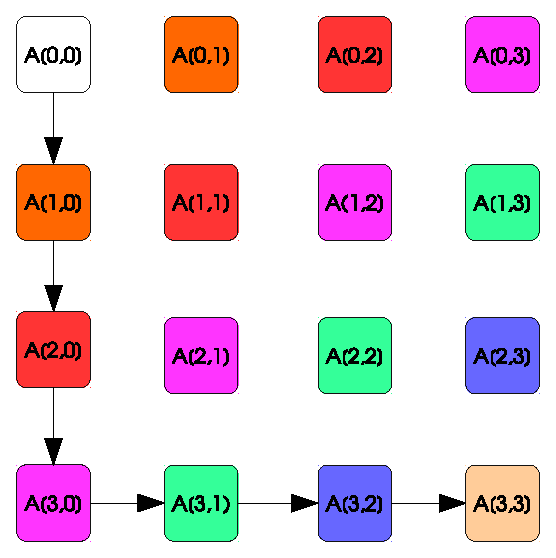
\includegraphics[scale=0.7]{seidelFlow.eps}
\end{figure}
Βλέπουμε ότι η Seidel Sor κάνει πολύ μεγάλο χρόνο σε σχέση με τις άλλες 2 μεθόδους κάτι που οφείλεται στον τρόπο που έχουμε επιλέξει να υλοποιήσουμε τον 
παραλληλισμό αλλά και στο γεγονός ότι περιμένει αρκετές "μελλοντικές" τιμές σε σχέση με την Jacobi πχ. 
Κοιτώντας τους χρόνους για ένα μοντέλο κατανεμημένης μνήμης θα διαλέγαμε τη μέθοδο Jacobi με tiles λόγω του μικρού χρόνου που κάνει.
\subsection*{Μετρήσεις χωρίς έλεγχο σύγκλισης}
Στο δεύτερο κομμάτι της εργασίας τρέξαμε για διάφορα μεγέθη πινάκων καθεμία από τις 3 μεθόδους για διαφορετικό συνολικό αριθμό OpenMP threads. Ακολουθούν τα 
ζητούμενα διαγράμματα:
\newpage
\clearpage
\begin{figure}
        \begin{subfigure}
                \includegraphics[scale=0.35]{scaletjb.png}
        \end{subfigure}
        \begin{subfigure}
                \includegraphics[scale=0.35]{scalesdl.png}
        \end{subfigure}
        \centering
        \begin{subfigure}
                \includegraphics[scale=0.35]{scalerbl.png}
        \end{subfigure}
\end{figure}
\begin{figure}
        \begin{subfigure}
                \includegraphics[scale=0.35]{barstjb512.png}
        \end{subfigure}
        \begin{subfigure}
                \includegraphics[scale=0.35]{barssdl512.png}
        \end{subfigure}
        \begin{subfigure}
                \includegraphics[scale=0.35]{barsrbl512.png}
        \end{subfigure}
        \begin{subfigure}
                \includegraphics[scale=0.35]{barstjb1024.png}
        \end{subfigure}
\end{figure}
\newpage
\clearpage
\begin{figure}
        \begin{subfigure}
                \includegraphics[scale=0.35]{barssdl1024.png}
        \end{subfigure}
        \begin{subfigure}
                \includegraphics[scale=0.35]{barsrbl1024.png}
        \end{subfigure}
        \begin{subfigure}
                \includegraphics[scale=0.35]{barstjb2048.png}
        \end{subfigure}
        \begin{subfigure}
                \includegraphics[scale=0.35]{barssdl2048.png}
        \end{subfigure}
        \centering
        \begin{subfigure}
                \includegraphics[scale=0.35]{barsrbl2048.png}
        \end{subfigure}
\end{figure}
\newpage
\clearpage
\section*{Σχολιασμός αποτελεσμάτων}
Στην tiled jacobi βλέπουμε ότι το speedup είναι περίπου γραμμικό εκτός από το μέγεθος 1024 που είναι σχεδόν τετραγωνικό διότι τότε τα tiles μας ταιριάζουν 
καλύτερη στην μνήμη. Στην Seidel Sor έχουμε υπογραμμικό speedup και παρατηρούμε κορεσμό στο τέλος πράγμα που φαίνεται και στα παρακάτω διαγραμματα διότι τρώμε
πολύ χρόνο στο συγχρονισμό των διεργασιών. Τέλος στην Red Black Sor δεν έχουμε tiles άρα δεν μπορούμε να κρίνουμε το speedup διότι ανάλογα με τον αριθμό των
threads μπορούμε να έχουμε καλύτερη συμμετρία ή να έχουμε καλύτερο διαμοιρασμό εργασιών αφού χωρίζουμε "οριζόντια" και "κάθετα" σε ορθογώνια ανάλογα με τα 
threads που εισάγουμε σε κάθε διάσταση.

Όσον αφορά το χρόνο υπολογισμών σε σχέση με το συνολικό χρόνο του προγράμματος βλέπουμε ότι πέρα από την Seidel SOR δεν έχουμε πολύ σημαντικές διαφορές. Η μεγάλη
διαφορά στην Seidel SOR οφείλεται στον διαγώνιο συγχρονισμό που πρέπει να έχει το πρόγραμμά μας. Οι άλλες 2 μέθοδοι έχουν η καθεμία το δικο της φόρτο και η 
επικοινωνία γίνεται σχεδόν άμεσα.
\end{document}
